% Homework template for Inference and Information
% UPDATE: September 26, 2017 by Xiangxiang
\documentclass[a4paper]{article}
\usepackage{ctex}
\usepackage{amsmath, amssymb, amsthm}
\usepackage{moreenum}
\usepackage{mathtools}
\usepackage{url}
\usepackage{bm}
\usepackage{enumitem}
\usepackage{graphicx}
\usepackage{listings}
\usepackage{color}

\lstset{
    basicstyle          =   \sffamily,          % 基本代码风格
    keywordstyle        =   \bfseries,          % 关键字风格
    commentstyle        =   \rmfamily\itshape,  % 注释的风格,斜体
    stringstyle         =   \ttfamily,  % 字符串风格
    flexiblecolumns,                % 别问为什么,加上这个
    numbers             =   left,   % 行号的位置在左边
    showspaces          =   false,  % 是否显示空格,显示了有点乱,所以不现实了
    numberstyle         =   \zihao{-5}\ttfamily,    % 行号的样式,小五号,tt等宽字体
    showstringspaces    =   false,
    captionpos          =   t,      % 这段代码的名字所呈现的位置,t指的是top上面
    frame               =   lrtb,   % 显示边框
}

\lstdefinestyle{Python}{
    language        =   Python, % 语言选Python
    basicstyle      =   \zihao{-5}\ttfamily,
    numberstyle     =   \zihao{-5}\ttfamily,
    keywordstyle    =   \color{blue},
    keywordstyle    =   [2] \color{teal},
    stringstyle     =   \color{magenta},
    commentstyle    =   \color{red}\ttfamily,
    breaklines      =   true,   % 自动换行,建议不要写太长的行
    columns         =   fixed,  % 如果不加这一句,字间距就不固定,很丑,必须加
    basewidth       =   0.5em,
}
\usepackage{subcaption}
\usepackage{booktabs} % toprule
\usepackage[mathcal]{eucal}
\usepackage[thehwcnt = 3]{iidef}

\thecourseinstitute{清华大学电子工程系}
\thecoursename{\textbf{媒体与认知} \space 课堂2}
\theterm{2021-2022学年春季学期}
\hwname{作业}
\begin{document}
\courseheader
\name{李智毅}
\vspace{3mm}
\centerline{\textbf{\Large{理论部分}}}

\section{单选题(15分)}
\subsection{\underline{D}}

\subsection{\underline{B}}

\subsection{\underline{D}}

\subsection{\underline{C}}

\subsection{\underline{B}}

\section{计算题(15 分)}
\subsection{
已知某卷积层的输入为$X$(该批量中样本数目为1,输入样本通道数为1),采用一个卷积核$W$,即卷积输出通道数为1,卷积核尺寸为$2\times 2$,卷积的步长为1,无边界延拓,偏置量为$b$:
$$X=\left[ \begin{array}{ccc}
    -0.5 & 0.2 & 0.3 \\
    0.6 & -0.4 & 0.1 \\
    0.4 & 0.5 & -0.2
\end{array}\right],
W=\left[ \begin{array}{cc}
    -0.2 & 0.1  \\
    0.4 & -0.3
\end{array}\right], b=0.05$$
}
\subsubsection{请计算卷积层的输出$Y$。}
直接计算
$$ Y_{11} = -0.5\times-0.2 + 0.2\times0.1 + 0.6\times0.4 + -0.4\times-0.3 + 0.05 = 0.53 $$
$$ Y_{12} = 0.2\times-0.2 + 0.3\times0.1 + -0.4\times0.4 + 0.1\times-0.3 + 0.05 = 0.15 $$
$$ Y_{21} = 0.6\times-0.2 + -0.4\times0.1 + 0.4\times0.4 + 0.5\times-0.3 + 0.05 = -0.1 $$
$$ Y_{22} = -0.4\times-0.2 + 0.1\times0.1 + 0.5\times0.4 + -0.2\times-0.3 + 0.05 = 0.4 $$
$$ Y=\left[ \begin{array}{cc}
    0.53 & -0.15 \\
    -0.1 & 0.4
\end{array}
\right]
$$

\subsubsection{若训练过程中的目标函数为$L$,且已知$\frac{\partial L}{\partial Y}=\left[ \begin{array}{cc}
    0.1 & -0.2 \\
    0.2 & 0.3
\end{array} \right]$,请计算$\frac{\partial L}{\partial X}$。
}
$$
\frac{\partial L}{\partial X} = 
\left[ \begin{array}{cc}
    -0.3 & 0.4 \\
    0.1 & -0.2
\end{array} \right] * 
\left[ \begin{array}{cccc}
    0 & 0 & 0 & 0 \\
    0 & 0.1 & -0.2 & 0 \\
    0 & 0.2 & 0.3 & 0 \\
    0 & 0 & 0 & 0
\end{array} \right] = 
\left[ \begin{array}{ccc}
    -0.02 & 0.05 & -0.02 \\
    0 & -0.15 & 0.09 \\
    0.08 & 0.06 & -0.09
\end{array} \right]
$$

注:本题的计算方式不限,但需要提供计算过程以及各步骤的结果。
\vspace{6mm}
\centerline{\textbf{\Large{编程部分}}}
\vspace{3mm}

% 请根据是否选择自选课题的情况选择“编程作业报告”或“自选课题开题报告”中的一项完成
\section{编程作业报告}
\subsection{完成程序代码}
按照要求,完成以下代码:\\
完成卷积层的实现,包括定义、前向计算、反向传播及参数初始化等;\\
按照要求使用nn.Sequential搭建网络结构;\\
使用ImageFolder构建数据集。\\

\subsection{训练与测试}
\subsubsection{默认参数}
训练轮数:10\\
验证集准确率收敛:90\%\\
测试集准确率:88.5\%\\
loss曲线(图1)\\
\begin{figure}
    \centering
    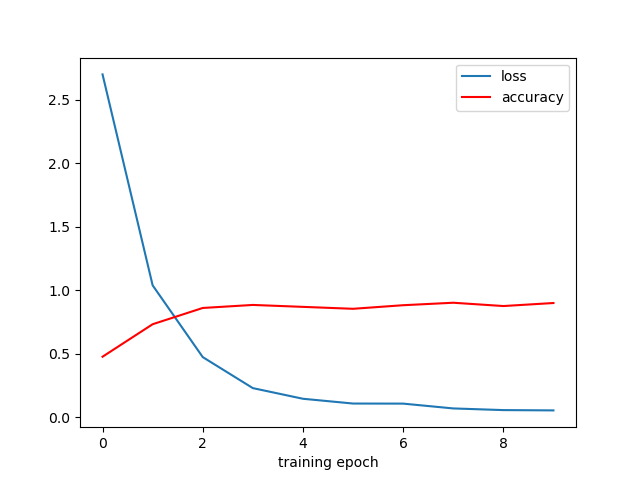
\includegraphics[width=12cm]{Fig1.png}
    \caption{默认参数训练}
\end{figure}

\subsubsection{启用batch normalization}
训练轮数:10\\
验证集准确率收敛:91\%\\
测试集准确率:91.5\%\\
loss曲线(图2)\\
对比默认参数:可以看出,在归一化处理之后,训练模型收敛更快,模型准确率也更高。\\
\begin{figure}
    \centering
    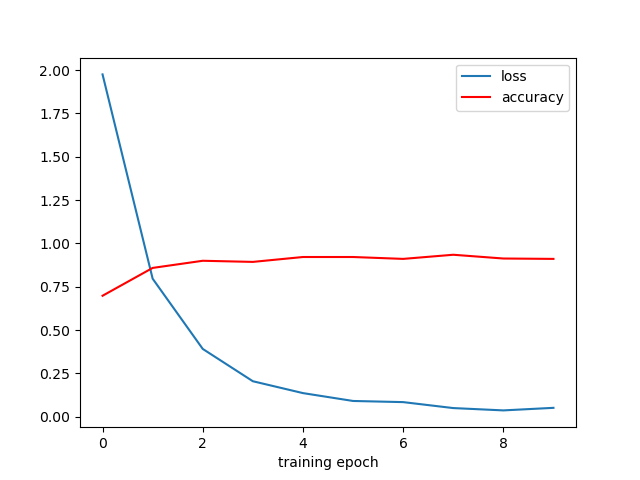
\includegraphics[width=12cm]{Fig2.png}
    \caption{启用batch normalization训练}
\end{figure}

\subsubsection{改变dropout概率为0.3}
训练轮数:10\\
验证集准确率收敛:88\%\\
测试集准确率:88.1\%\\
loss曲线(图3)\\
对比默认参数:可以看出,在使用dropout之后,模型准确率并没有明显提升。\\
\begin{figure}
    \centering
    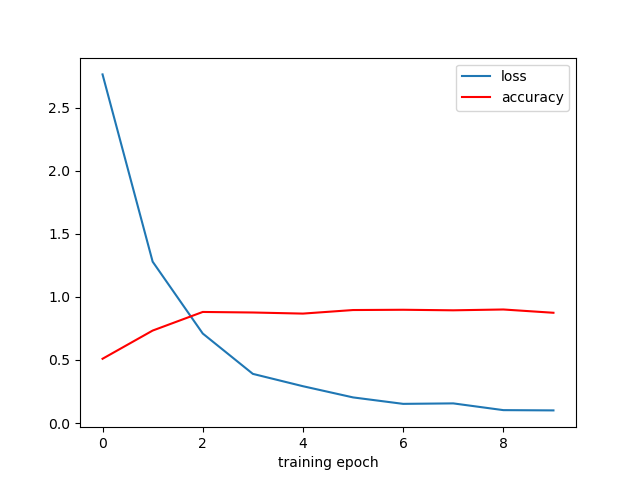
\includegraphics[width=12cm]{Fig3.png}
    \caption{改变dropout概率为0.3训练}
\end{figure}

\subsection{可视化}
选择第二个模型(归一化训练模型),结果如下\\
\subsubsection{可视化第0层卷积层卷积核}
可视化第0层卷积层卷积核(图4)\\
\begin{figure}
    \centering
    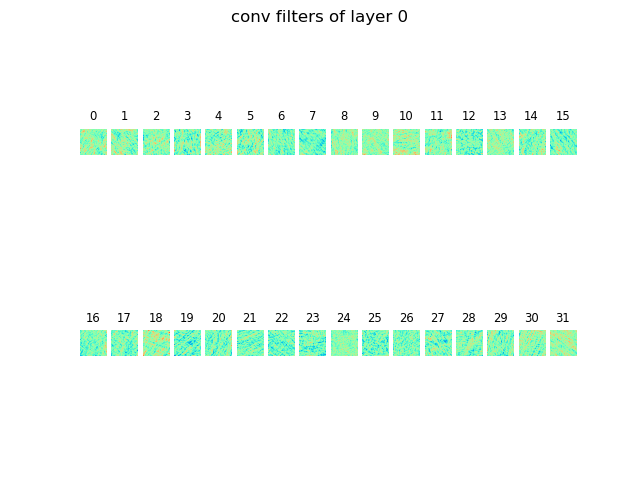
\includegraphics[width=12cm]{Fig4.png}
    \caption{可视化第0层卷积层卷积核}
\end{figure}

\subsubsection{可视化第100张图像第1层卷积层的输出特征图}
可视化第100张图像第1层卷积层的输出特征图(图5)\\
\begin{figure}
    \centering
    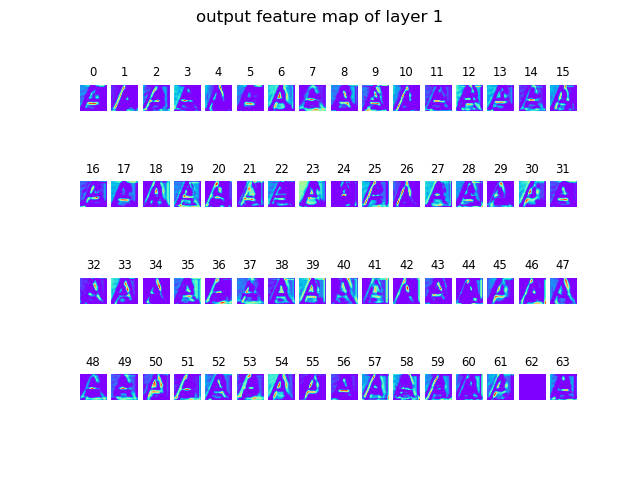
\includegraphics[width=12cm]{Fig5.png}
    \caption{可视化第100张图像第1层卷积层的输出特征图}
\end{figure}

\subsubsection{t-SNE显示分类结果}
t-SNE显示分类结果(图6)\\
\begin{figure}
    \centering
    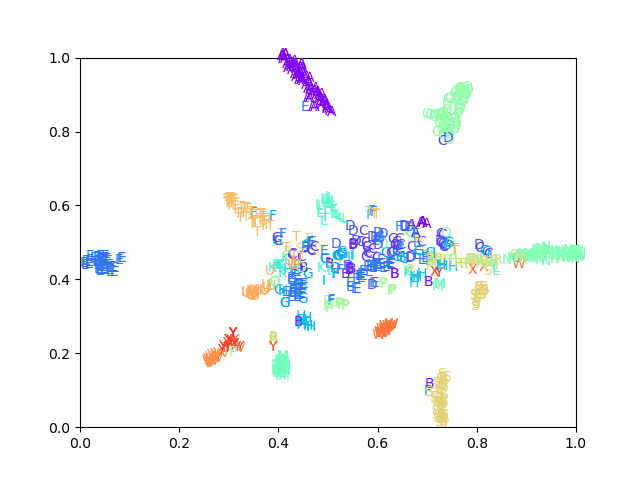
\includegraphics[width=12cm]{Fig6.png}
    \caption{t-SNE显示分类结果}
\end{figure}

\subsection{熵计算}
\subsubsection{单张图像熵计算}
选取的图像为"data/test/E/1431.jpg",字母为"E"(图7)\\
\begin{figure}
    \centering
    \includegraphics[width=2cm]{../data/test/E/1431.jpg}
    \caption{熵计算选取的图像}
\end{figure}
使用模型:bn\_ckpt,即正则化之后的训练模型\\
识别结果:E\\
置信度:0.98\\
图像熵:4.88\\
特征熵:3.16, 2.86, 4.03, 2.55, 3.47\\
预测概率熵:0.14\\
可以看出,该模型对于此图像的预测较为准确,置信度较高,说明该模型对此类分类问题应用较好。\\

\subsubsection{测试集熵计算}
测试集图像熵:4.11\\
特征熵:3.05, 3.03, 4.08, 2.59, 3.51\\
随机猜测熵(每个字符概率为 $ \frac{1}{26} $ ):3.26\\
训练集label熵:2.93\\
模型预测概率熵:0.46\\
可以看出,在使用模型预测之后,对比随机猜测,熵降低了许多,这说明模型对此类分类问题提供的信息较为准确有效。\\

\subsection{实验小结}
遇到的困难:卷积层的实现,特别是维度匹配问题以及fold、unfold函数使用问题。\\
解决方案:根据卷积展开计算的方法,按照维度仔细地正确使用torch.matmul函数及fold、unfold函数。\\

\end{document}



%%% Local Variables:
%%% mode: late\rvx
%%% TeX-master: t
%%% End:
